% !TEX TS-program=xelatex
\documentclass{../../templates/information_retrieval_lab}
\pagestyle{plain}
\begin{document}

% file for general details about your work
\newcommand{\reportAuthor}{Косенко Олександр Володимирович}
%\newcommand{\reportSupervisor}{}
\newcommand{\reportAuthorGroup}{КП-11}
\newcommand{\reportYear}{2025}


\newcommand{\labNo}{2}

\newcommand{\labTopic}{РЕАЛІЗАЦІЯ АЛГЕБРАЇЧНОЇ МОДЕЛІ ПОДАННЯ ДОКУМЕНТІВ}

\thispagestyle{empty}
\setlength{\parindent}{0cm}

\begin{center}
МІНІСТЕРСТВО ОСВІТИ І НАУКИ УКРАЇНИ

НАЦІОНАЛЬНИЙ ТЕХНІЧНИЙ УНІВЕРСИТЕТ УКРАЇНИ

«КИЇВСЬКИЙ ПОЛІТЕХНІЧНИЙ ІНСТИТУТ ІМЕНІ ІГОРЯ СІКОРСЬКОГО»

\vfill

Факультет прикладної математики

Кафедра програмного забезпечення комп’ютерних систем

\vfill

\textbf{Лабораторна робота №\labNo}

з дисципліни «Програмне забезпечення інформаційно-пошукових систем»

тема «\labTopic»
\end{center}

\vfill

{\renewcommand{\arraystretch}{0.7}
\begin{tabularx}{\textwidth}{>{\setlength\hsize{1\hsize}}X >{\setlength\hsize{1\hsize}}X}
&Виконав cтудент\\                                         % & \\
&студент IV курсу групи \reportAuthorGroup\\               % & \\
&\reportAuthor\\                                           % & \rule{2.5cm}{0.25pt}   \\[6pt]
%Керівник:                                                & \\
%\supervisorRegalia                                       & \\
%\supervisorFio                                           & \rule{2.5cm}{0.25pt}   \\[6pt]
%%%%% Якщо у вас є консультант у роботі - розкоментуйте наступні три рядки (а цей - не розкоментовуйте!)
%Консультант:                                             & \\
%\consultRegalia                                          & \\
%\consultFio                                              & \rule{2.5cm}{0.25pt}   \\[6pt]
%Рецензент:                                               & \\
%\reviewerRegalia                                         & \\
%\reviewerFio                                             & \rule{2.5cm}{0.25pt} 
\end{tabularx}
}

\vfill

\centerline{КИЇВ \reportYear}

\setlength{\parindent}{1.25cm}

\pagebreak


\centerline{\textbf{Постановка задачі}}

Реалізувати інформаційно-пошукову систему, що використовує векторно-
просторову модель подання документів, відповідно до наступних вимог:

1. Для реалізації інформаційно-пошукової системи може
використовуватись будь-який стек (мова програмування, фреймворк і
так далі) технологій.

2. Інформаційно-пошукова система може мати будь-який з перелічених
інтерфейсів користувача: консольний, веб, мобільний, настільний.

3. Розроблена інформаційно-пошукова система має використовувати
векторно-просторову модель подання документів.

4. Міра tf-idf, необхідна для реалізації векторно-просторової моделі,
визначається відповідно до варіанту студента (див. Додаток Б).

5. Для обчислення подібності між документами та пошуковими запитами
необхідно використати косинусну міру. Граничне значення подібності, за якої документ повинен відображатися у результатах запиту,
обирається студентом самостійно.

6. Робота з розробленою інформаційно-пошуковою системою має бути
поділена на наступні етапи:

a. Введення колекції документів.

i. Користувач повинен мати можливість ввести будь-яку
невід’ємну кількість документів (хоча б один документ у колекції
є обов’язковим).

ii. Допускається (на вибір студента) реалізація введення колекції
документів за допомогою її зчитування з окремих текстових
файлів, розміщених у певній директорії (один текстовий файл =
один документ). У такому випадку, на даному етапі користувач
вводить шлях до директорії з файлами.

iii. Документи складаються з термів, розділених пробілами (без
знаків пунктуації), та написаних символами лише нижнього
регістру.

iv. Після закінчення введення, користувач автоматично переходить
на наступний етап.

b. Виконання пошукових запитів.

i. На даному етапі користувач вводить пошуковий запит і
переглядає його результати.

ii. При показі результатів запиту потрібно обов’язково вивести
обчислене значення подібності для кожного документа.

iii. Після виконання пошукового запиту, користувач повинен
залишатися на цьому ж етапі, з можливістю ввести новий
пошуковий запит.

Для варіанту $9$: $tf=\log(1+f_{t,d})$, $idf=1$

\centerline{\textbf{Хід роботи}}

Лістинг 1. Реалізація пошуку за векторним представленням документів

\lstinputlisting[language=python, style=minimalist]{../program/src/main.py}

У даній програмі представлення документів є словником, у якому ключами є терми, що містяться в документі, а значеннями - відповідні $tf$. При обчисленні косинусної подібності векторний добуток обчислюється як:

\begin{equation*}
sim(d,q)=\frac{\sum\limits_{t\in d\cap q}tf_{t,d}\cdot tf_{t,q}}{\sqrt{\sum\limits_{t\in d}tf_{t,d}^2}\cdot\sqrt{\sum\limits_{t\in q}tf_{t,q}^2}}
\end{equation*}

При отриманні результату повертаються ті документи, подібність представлення яких не менша порогового значення, яке може бути змінене користувачем. Крім того, користувач може задати максимальну кіклькість документів у відповіді, а також додавати до індексу нові файли.

\centerline{\textbf{Результати роботи}}

Для демонстрації результату створимо документи поділивши на чатини статтю з Вікіпедії (\url{https://en.wikipedia.org/wiki/C_(programming_language)}), прибравши з тексту все що не є літерами та пробілами та звівши всі літери до малих.

\begin{figure}[H]
    \centering
    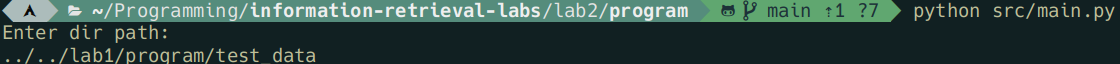
\includegraphics[width=\textwidth]{img/screen0.png}
    \caption{Введення шляху до документів}
\end{figure}

\begin{figure}[H]
    \centering
    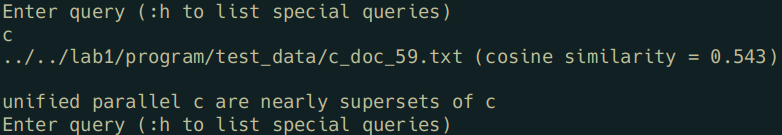
\includegraphics[width=\textwidth]{img/screen1.png}
    \caption{Виконання пошукового запиту}
\end{figure}

\begin{figure}[H]
    \centering
    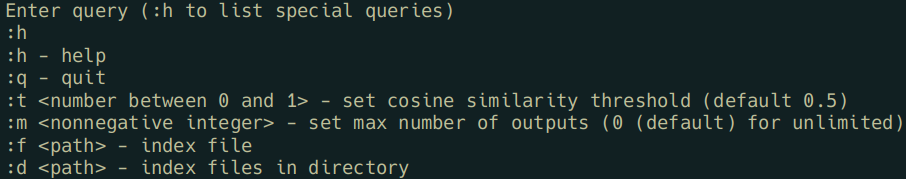
\includegraphics[width=\textwidth]{img/screen2.png}
    \caption{Виведення спеціальних запитів}
\end{figure}

\begin{figure}[H]
    \centering
    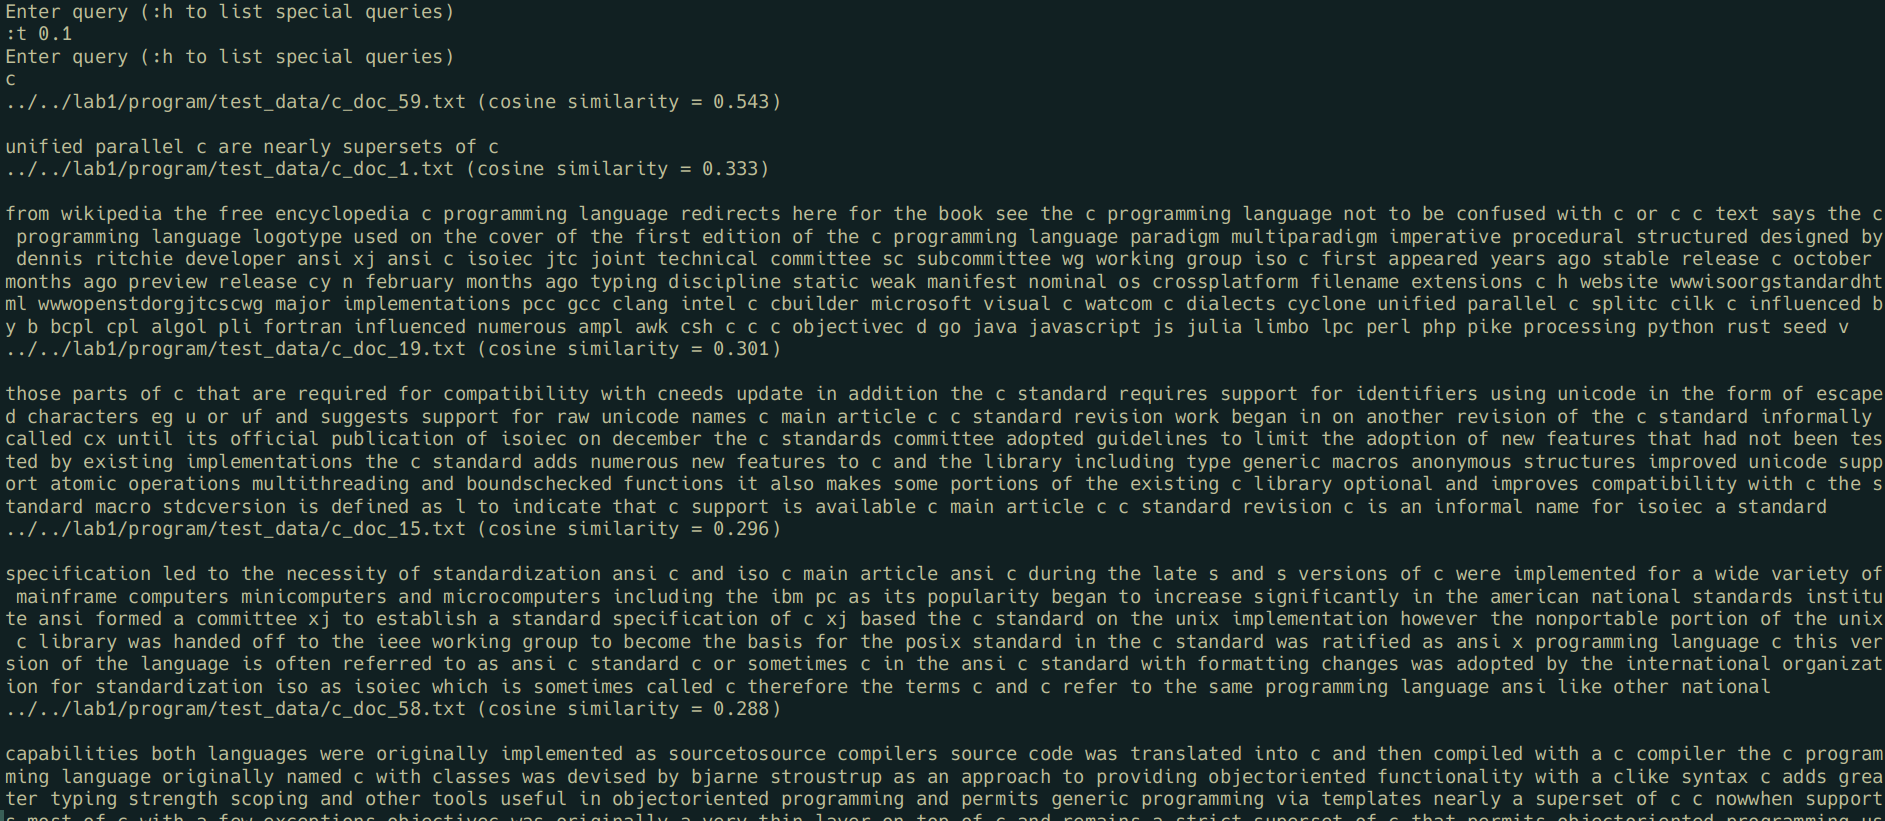
\includegraphics[width=\textwidth]{img/screen3.png}
    \caption{Зміна порогового значення подібності}
\end{figure}

\begin{figure}[H]
    \centering
    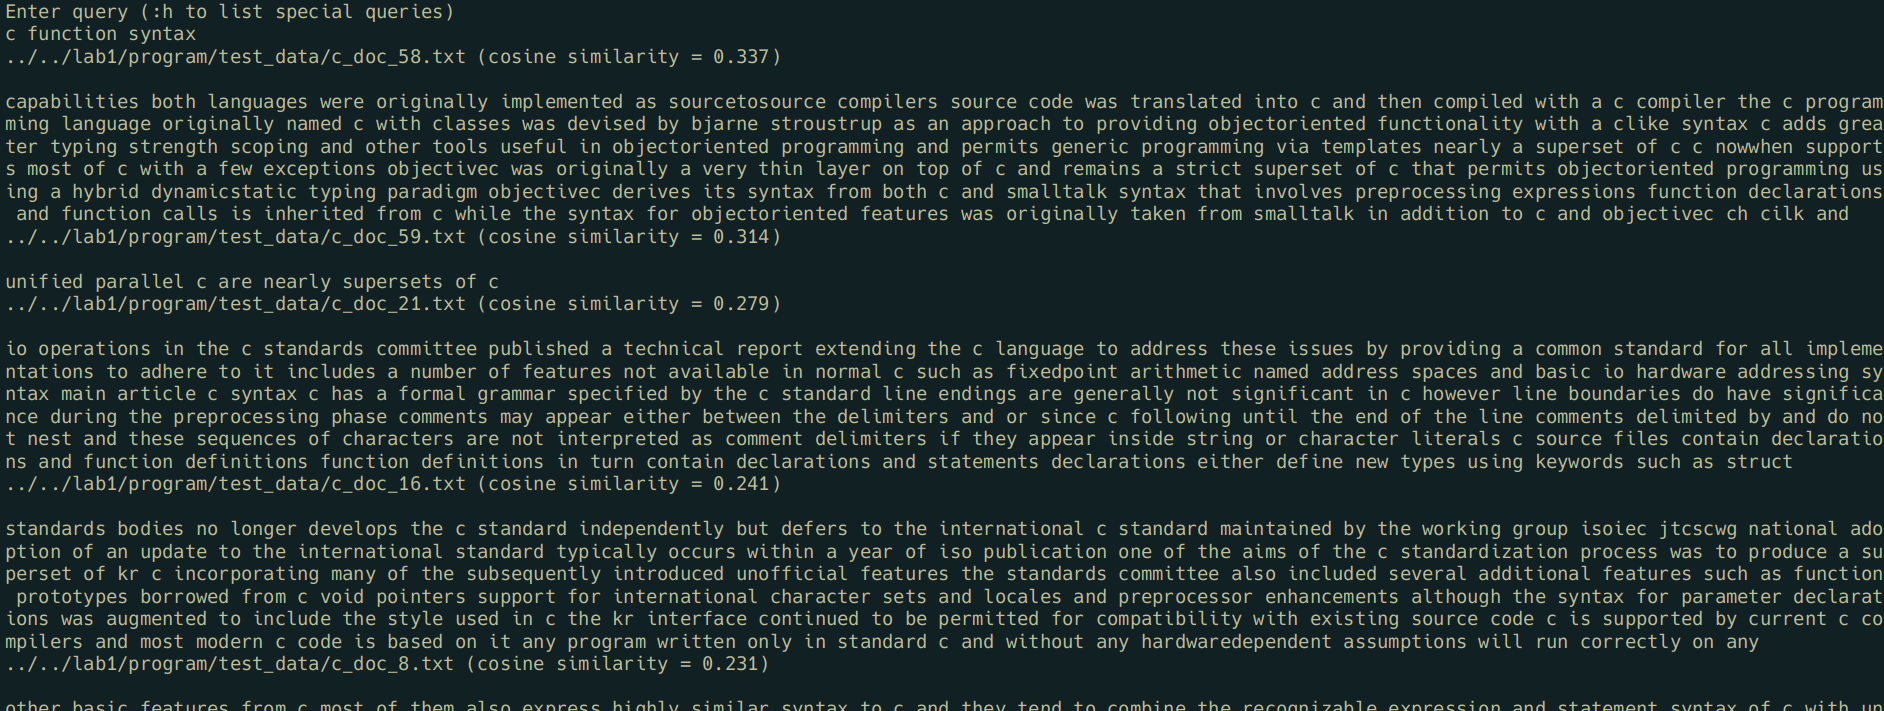
\includegraphics[width=\textwidth]{img/screen4.png}
    \caption{Запит з кількох слів}
\end{figure}

\begin{figure}[H]
    \centering
    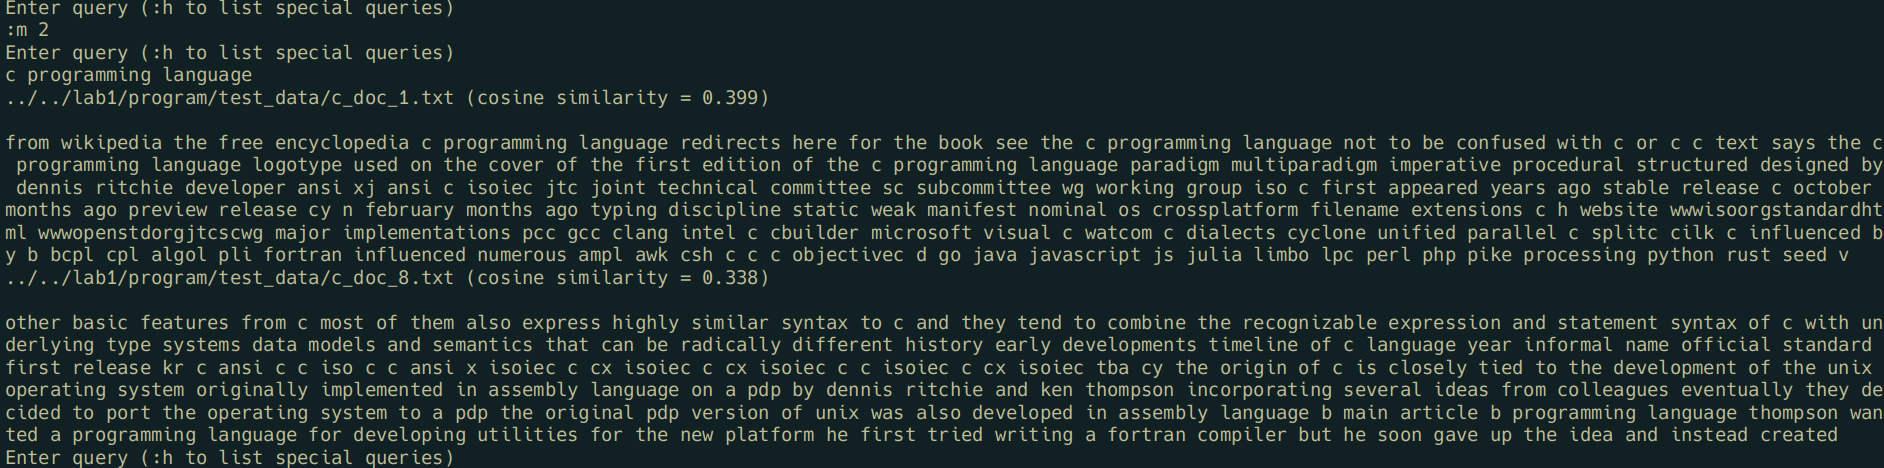
\includegraphics[width=\textwidth]{img/screen5.png}
    \caption{Встановлення максимальної кількості документів}
\end{figure}

\begin{figure}[H]
    \centering
    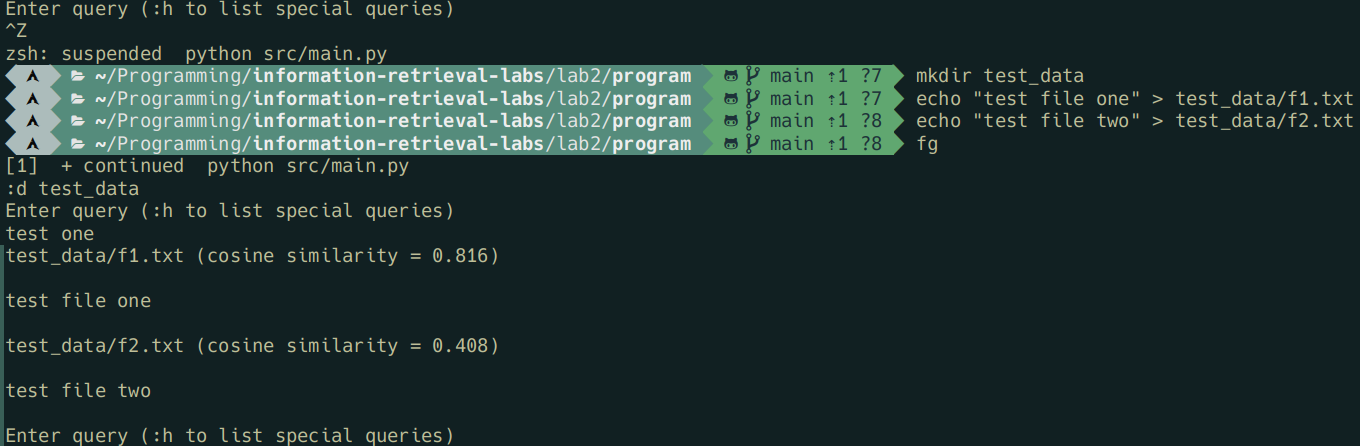
\includegraphics[width=\textwidth]{img/screen6.png}
    \caption{Додавання документів до індексу}
\end{figure}

\textbf{Висновки:} у ході виконання даної лабораторної роботи реалізовано пошукову систему на основі алгебраїчної моделі подання документів. Документи представлено векторами, кожен елемент яких відповідає деякому терму. Пошук та сортування документів проводяться за мірою подібності векторак запиту та документів.

\end{document}
